\section{方法}
\label{sec:method-zh}

\subsection{问题定义与方法概览}

给定包含镜头切换的单目视频流 $\{I_t\}_{t=1}^{T}$，\method{} 按时间顺序预测相机姿态 $C_t$ 和多个人体 $\mathcal H_t$，同时维护递归状态 $S_t$。连续镜头内，状态提供稳定的时空参照。在镜头切换处，先前状态可以为建立两个镜头之间的关系提供参照；然而，继续传播该状态可能在新镜头内引入相机漂移，而单独重新初始化又会丢失跨镜头参照。

图像编码器将 $I_t$ 映射为 token $F_t$，检测到的人物由提示 $H_t$ 表示。它们与初始相机 token $p_0$ 一起，通过解码器 $D_\theta$ 和前一时刻状态交互：
\begin{equation}
 [F'_t,p_t,H'_t],S_t=D_\theta([F_t,p_0,H_t],S_{t-1}).
 \label{eq:stateful-reconstruction-zh}
\end{equation}
更新后的 token 预测相机局部坐标系中的场景点图 $P_t^c$、camera-to-world 相机姿态以及每个可见人物的 SMPL-X 参数；在齐次坐标下，世界坐标场景点图为 $P_t^w=C_tP_t^c$。

我们将上述在线映射简写为
\begin{equation}
 (y_t,S_t)=f_\theta(I_t,S_{t-1}),\qquad
 y_t=\left(C_t,P_t^w,\{J_t^i,V_t^i,q_t^i\}_{i=1}^{N_t}\right),
 \label{eq:online-map-zh}
\end{equation}
其中 $J_t^i$、$V_t^i$ 和 $q_t^i$ 分别为人物 $i$ 的 SMPL-X
~\citep{pavlakos2019smplx}
关节、网格顶点和匿名人物槽位。我们用预训练 \humanthree{} 实例化 $f_\theta$；它的状态联合表示相机、场景几何和人物
~\citep{chen2026human3r}。本文关注的是：当 $I_t$ 不再是 $S_{t-1}$ 所表示视频流的连续观测时，应如何转换状态并统一输出坐标。

\method{} 将镜头间对齐与递归状态传播分离。在检测到的边界 $b$，同一帧首先结合前一状态估计镜头间关系，同时从空状态独立初始化后续递归：
\begin{equation}
\begin{aligned}
 (\widetilde y_b,\widetilde S_b)&=f_{\theta,\phi}(I_b,S_{b-1}), &
 (y_b^r,S_b^r)&=f_\theta(I_b,S_{\varnothing}).
\end{aligned}
\label{eq:boundary-paths-zh}
\end{equation}
边界之后只传播 $S_b^r$。人物关联与共享变换进一步维持世界坐标和身份一致性（图~\ref{fig:method-zh}）。

\begin{figure*}[t]
  \centering
  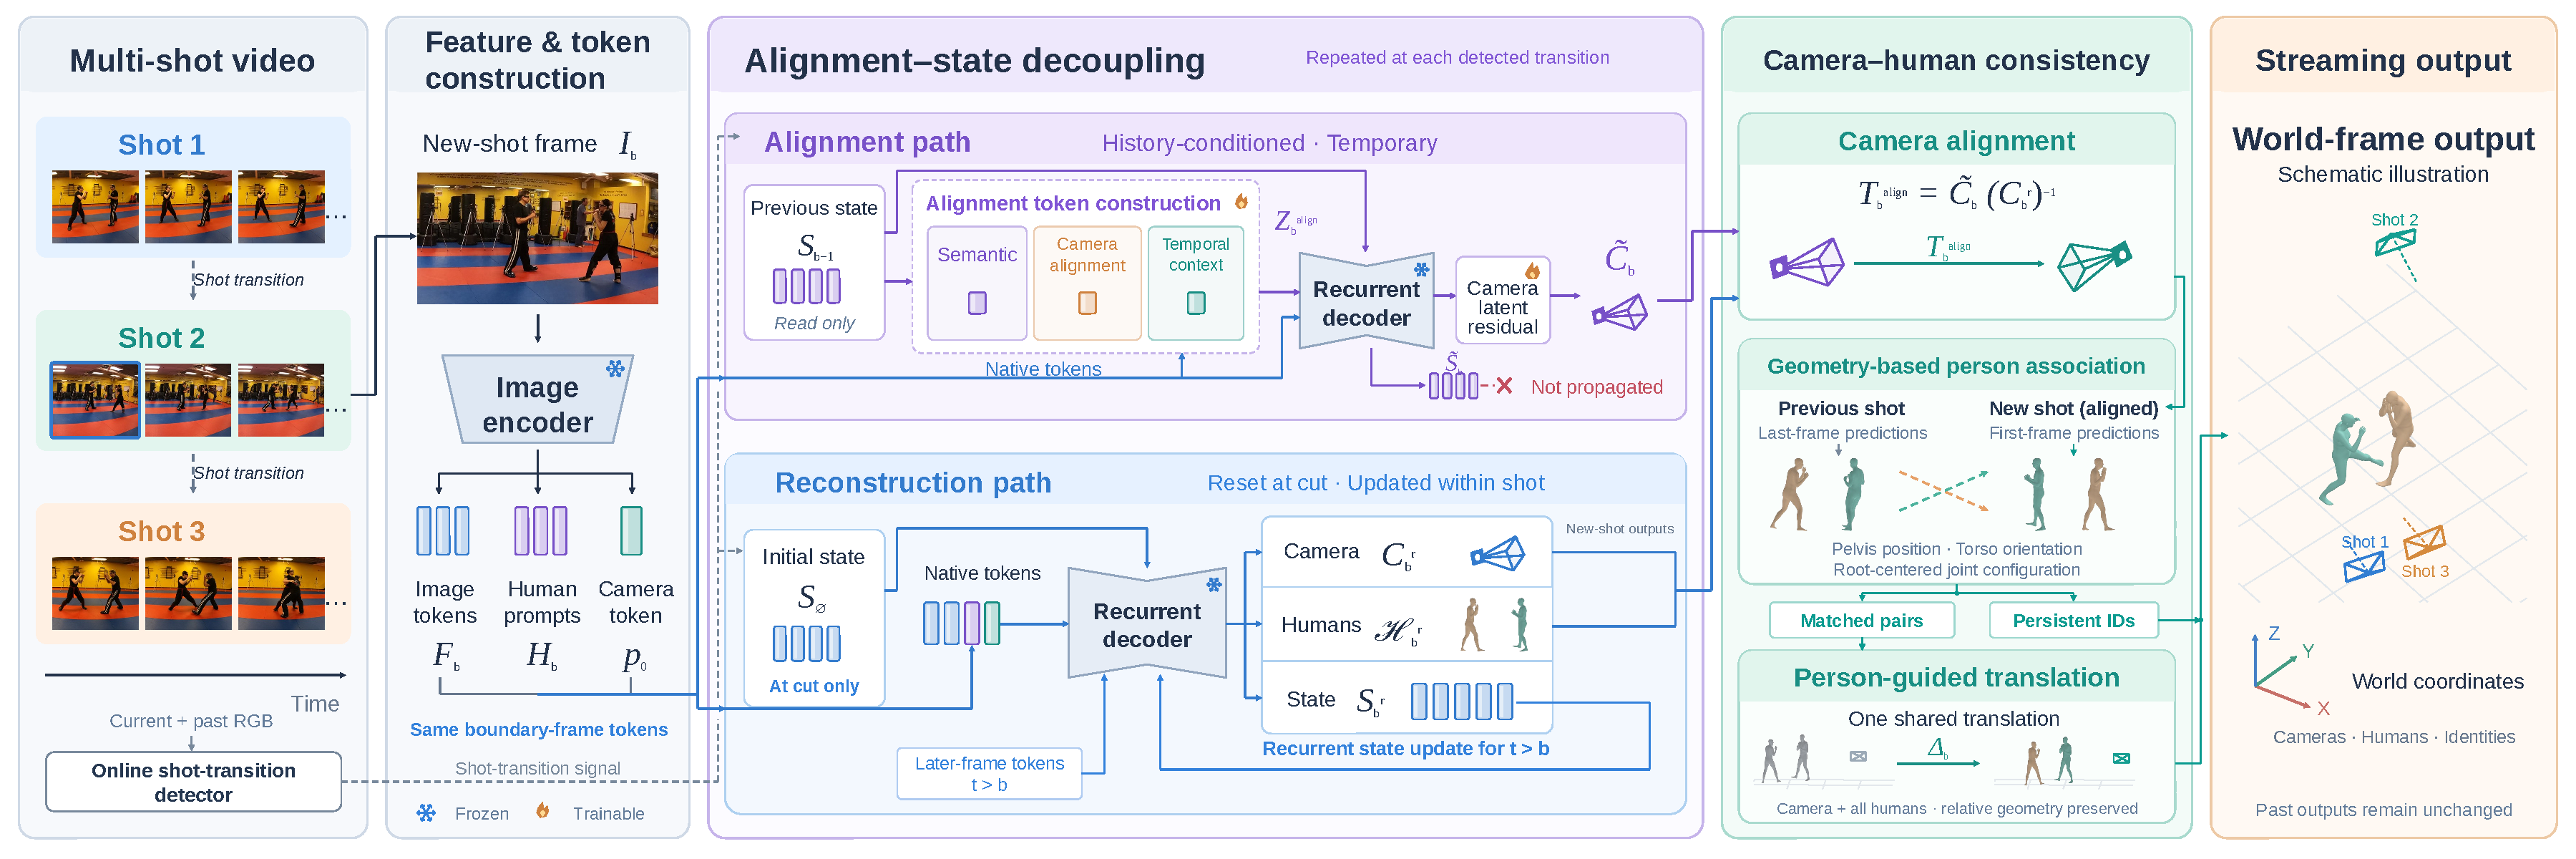
\includegraphics[width=\textwidth]{figures/method.pdf}
  \caption{\method{} 方法概览。历史条件路径估计镜头间对齐，而只有重新初始化路径传播递归状态。基于几何的跨镜头人物关联连接人物身份，共享变换将相机、人体和世界坐标场景点映射到已有世界坐标系。最右侧输出面板为示意图。}
  \label{fig:method-zh}
\end{figure*}

\subsection{历史条件镜头对齐}

在线镜头切换检测器只利用当前与历史 RGB 定位新镜头首帧 $b$。它仅决定何时启动对齐，不估计空间变换或人物对应关系，也不访问未来帧、相机标定或人体标注；完整结构和触发策略见英文补充材料。

在检测到的边界，镜头对齐模块 $\Phi_\phi$ 建立当前观测与上一镜头状态之间的联系。语义、相机对齐和时间上下文三种带类型的 token 分别表示当前与历史之间的视觉证据、潜在相机变化和此前的校正上下文，并与冻结主干的原生 token 一同解码。注意力汇聚首先得到当前证据 $c_b$ 与历史记忆 $m_{b-1}$：
\begin{equation}
\begin{aligned}
 z_b^{\mathrm{sem}}&=\alpha_b c_b+(1-\alpha_b)m_{b-1}, &
 z_b^{\mathrm{cam}}&=\operatorname{MLP}_{\mathrm{cam}}[p_b,p_{b-1},\Delta p_b,m_{b-1}],\\
 z_b^{\mathrm{temp}}&=\operatorname{MLP}_{\mathrm{temp}}[\bar z_{b-1},\delta_{b-1},g_{b-1}], &
 Z_b^{\mathrm{align}}&=[z_b^{\mathrm{sem}},z_b^{\mathrm{cam}},z_b^{\mathrm{temp}}].
\end{aligned}
\label{eq:alignment-tokens-zh}
\end{equation}
\noindent
\begin{minipage}[t]{0.57\textwidth}
\vspace{0pt}
其中，$\alpha_b$ 融合当前与历史语义证据；$p$、$\bar z$、$\delta$ 和 $g$ 分别表示相机 token、前一次对齐摘要、相机潜变量残差及其门控值。三种表示与人体潜变量残差分支共同使边界预测适应已有世界参照，并给出临时相机估计 $\widetilde C_b$；汇聚和残差分支的完整定义见英文补充材料。

\smallskip
我们从共享世界坐标下的动态人体采集中构造四帧序列。镜头切换序列遵循 $A(t),A(t+1),B(t+2),B(t+3)$，连续序列则取同一相机的四帧；前者监督镜头间变化，后者抑制连续输入中的不必要校正。
\end{minipage}\hfill
\begin{minipage}[t]{0.39\textwidth}
  \vspace{0pt}
  \centering
  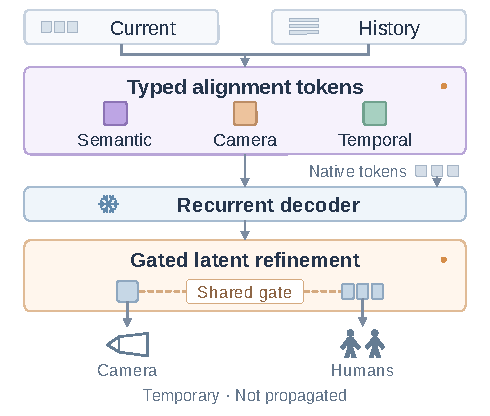
\includegraphics[width=0.94\linewidth]{figures/alignment_module.pdf}
  \captionof{figure}{\textbf{镜头对齐模块。}带类型的 token 关联当前与历史证据；门控残差不向后传播。}
  \label{fig:alignment-module-zh}
\end{minipage}

\medskip
对齐训练目标为
\begin{equation}
 \mathcal L_{\mathrm{align}}=\mathcal L_t+5\mathcal L_R+10\mathcal L_h
 +0.05(\mathcal L_g+\mathcal L_{\mathrm{imp}})
 +10^{-5}(\mathcal R_{\mathrm{cam}}+\mathcal R_{\mathrm{human}}),
 \label{eq:alignment-objective-zh}
\end{equation}
其中 $\mathcal L_t$ 与 $\mathcal L_h$ 为相机和人体平移的 Smooth-L1 损失，$\mathcal L_R$ 为四元数测地距离。令 $e$ 和 $e^{\mathrm{raw}}$ 分别表示归一化后的校正相机误差与未校正误差，则
$\mathcal L_g=\operatorname{BCE}(g,\operatorname{clip}(e^{\mathrm{raw}},0,1))$，
$\mathcal L_{\mathrm{imp}}=[e-e^{\mathrm{raw}}]_+$。

仅三种对齐 token、相机与人体潜变量残差分支，以及预测头中的低秩适配参数
~\citep{hu2022lora}
参与训练，共 19.62M 参数，占完整模型的 1.63\%。图像编码器、递归主干、基础预测头和 Multi-HMR 组件
~\citep{baradel2024multihmr}
均保持冻结。这些参数位于历史与当前观测的接口处，用于学习镜头关系，而不重新学习镜头内部重建。

\subsection{分离对齐与状态传播}

式~\ref{eq:boundary-paths-zh} 中两次边界计算具有不同的信息生命周期。历史条件状态 $\widetilde S_b$ 只临时使用，新镜头后续帧仅由重新初始化路径递归更新：
\begin{equation}
 (y_t^r,S_t^r)=f_\theta(I_t,S_{t-1}^r),\qquad t>b.
\label{eq:dual-path-zh}
\end{equation}
因此，历史能够在边界建立明确的空间关系，却没有递归通路进入新镜头的后续状态。

重新初始化路径根据同一图像预测 $C_b^r$。两条路径观察相同内容但历史条件不同，因此二者的相对相机变换可将新镜头对齐到已有世界坐标系：
\begin{equation}
 T_b^{\mathrm{align}}=\widetilde C_b(C_b^r)^{-1}.
 \label{eq:inter-shot-alignment-zh}
\end{equation}
形成该变换后，历史条件路径的全部临时预测和 $\widetilde S_b$ 均被丢弃。后续镜头切换独立重复这一操作，且不修改已输出结果。

\subsection{跨镜头相机与人体一致性}

$T_b^{\mathrm{align}}$ 首先将重新初始化路径的相机和人体预测映射到前一镜头的世界坐标系。由于相机对齐本身不能确定人物身份，\method{} 使用预测的骨盆位置、躯干朝向和去根节点平移后的关节结构进行一对一匹配：
\begin{equation}
 d_{ij}=\widehat d_{\mathrm{root}}(i,j)+
        \widehat d_{\mathrm{torso}}(i,j)+
        \widehat d_{\mathrm{joint}}(i,j).
 \label{eq:association-cost-zh}
\end{equation}
三个代价在 Hungarian assignment
~\citep{munkres1957assignment}
之前分别用其中位数归一化。匹配不使用身份标注、相机标定或未来帧；未匹配的新检测结果获得新的匿名身份。

对于匹配的前一镜头骨盆位置 $r_{b-1}^i$ 和完成相机对齐的新镜头位置 $\bar r_b^j$，鲁棒的共享平移为
\begin{equation}
 \Delta_b=\lambda\underset{(i,j)\in\mathcal M_b}{\operatorname{median}}
 (r_{b-1}^i-\bar r_b^j),\qquad \lambda=0.5.
 \label{eq:shared-translation-zh}
\end{equation}
固定系数 $\lambda$ 在仅相机对齐和完整人物位移之间进行插值，并在所有数据集上保持不变。历史条件路径的相机确定方向和初始世界关系，匹配人物的位移进一步调整共享平移，同时保持相机—人体相对几何不变。

令 $T_b^\Delta=\begin{bmatrix}I_3&\Delta_b\\\mathbf 0^\top&1\end{bmatrix}$ 且 $T_b=T_b^\Delta T_b^{\mathrm{align}}$，最终输出为
\begin{equation}
 C'_t=T_bC_t^r,\quad P_t^{\prime w}=T_bP_t^{r,w},\quad
 J_t^{\prime i}=T_bJ_t^{r,i},\quad V_t^{\prime i}=T_bV_t^{r,i},\quad
 q_t^{\prime i}=\pi_b(q_t^{r,i}),\quad S'_t=S_t^r.
 \label{eq:shared-world-transform-zh}
\end{equation}
因此，相机、世界坐标场景点和人体共享同一个世界变换；相机局部点图不发生形变，递归状态既不接受该变换，也不从前一镜头复制。后续每个边界都相对于累积世界坐标系估计新的变换；组合变换只影响当前与未来输出，已经输出的帧保持不变。
